%---------------------------------------------------------------------------%
%-                                                                         -%
%-                      论文整体框架                                        -%
%-                                                                         -%
%---------------------------------------------------------------------------%
%->> 论文基本信息(自行修改)
%---------------------------------------------------------------------------%
%论文标题
\def\theTitle{曲师大本科生毕业论文(理科)\LaTeX 模板}
\def\theEngTitle{The \LaTeX  plate for the bachelor thesis of Qufu Normal University}
%专业名称
\def\theMajor{数学与应用数学师范专业(师范)}
\def\theEnMajor{Mathematics and Applied Mathematics}
%院系
\def\theInstitution{数学科学学院}
%学号
\def\theNo{2015100013}
%作者姓名
\def\theAuthor{张三}
\def\theEnName{Zhang San}
%指导教师姓名
\def\theTutor{李四}
\def\theEnTutor{Li Si}
%指导教师职称
\def\theProTitle{讲师}
%论文定稿时间
\def\theDate{2019年5月15日}
%摘要
\def\theSummary{本文作者制作了对应曲阜师范大学本科生毕业论文(设计)的\LaTeX 模板, 本文给出了该模板的一些使用说明,  列举了一些\LaTeX 的具体使用例子.}
\def\theSummaryen{BlablaBlablaBlablaBlablaBlabla}
%关键词
\def\theKeywords{\LaTeX\   本科生毕业论文\    论文写作} 
\def\theKeywordsen{Aa;  Bb;  Cc;  Dd;  Ee} 
%---------------------------------------------------------------------------%
%->> 论文整体框架(按需引入/增删各章节)
%---------------------------------------------------------------------------%
\makecover % 封面
\makecontents % 目录
\makeheader % 标题/摘要
\section{引言}

毕业论文(设计)是专业人才培养方案的重要组成部分, 是学程即将结束时, 学生运用已学知识、理论和技能研究和解决问题的一次综合训练. 毕业论文(设计)在培养大学生探求真理、强化社会意识、进行科学研究基本训练、提高综合实践能力与素质等方面, 具有不可替代的作用, 是教育与生产劳动和社会实践相结合的重要体现, 是培养大学生的创新能力、实践能力和创业精神的重要实践环节.

目前, 学校的教务部门提供了本科生毕业论文(设计)的Word模板, 规定了论文写作的一系列格式. 然而, 在数学论文的排版方面, \LaTeX 系统比Word更有优势. \LaTeX 是\TeX 排版引擎的封装, 具有方便而强大的数学公式排版能力, 很容易生成复杂的专业排版元素, 如脚注、交叉引用、参考文献、目录等. 绝大多数时候, \LaTeX 用户只需专注于一些组织文档结构的基础命令, 无需(或很少)操心文档的版面设计. 为了配合数学专业本科生的毕业论文(设计)写作, 本文作者按照曲阜师范大学本科生毕业论文(设计)格式的要求, 制作了对应的\LaTeX 模板.

本文结构如下: 第2节, 我们给出模板的使用说明, 包含一些重要的注意事项. 第3节, 我们列举了一些常用的\LaTeX 使用例子.

 % 引言
\section{模板的使用说明}

将模板的压缩包下载,解压缩, 其中包括以下7项:
\begin{itemize}
  \item 文件夹cover, 用于存放封面的封面的\TeX 源文件和校徽、校名图片, 不建议使用者改动该文件夹.
  \item 文件夹Img, 用于存放论文中需要的插图.
  \item  thesis\_bachelor\_qfnu\_v1.tex, 这是tex源文件, 论文内容全部在该文件中输入.
  \item  qfnu\_BA\_bachelor.sty, 这是格式文件, 包含论文的版面格式、数学公式、章节格式、定理环境等相关的宏包和命令, 不建议使用者改动该文件.
  \item 曲阜师范大学本科毕业论文(设计)相关表格.doc, 包含毕业论文工作程序、撰写规范、详细的Word模板和相关表格. 可以用该文件填写相关表格.
  \item 说明.pdf, 本模板的说明文档.
  \item 校字〔2008〕89号-曲阜师范大学本科毕业论文(设计)工作管理办法.pdf, 学校文件, 包含毕业论文的规定、工作程序、撰写规范、Word模板和相关表格.

\end{itemize}
在编译thesis\_bachelor\_qfnu\_v1.tex文件时, 需要调用qfnu\_BA\_bachelor.sty格式文件和covers, Img文件夹, 因此应当它们始终处于同一个目录(文件夹)下. 一般情况下, 编译两次才能生成完整的pdf文件.

注意, 本模板要在TexLive系统下编译.

论文的作者只需要在tex源文件相应位置输入以下内容:
\begin{itemize}
  \item 自定义命令. 有些命令比较长但是需要在论文中频繁用到, 有时候一些符号并不在系统中, 此时作者可以按照一定的格式自定义一些新的命令. 见图\ref{pic: redefine}.
\begin{figure}
\centering
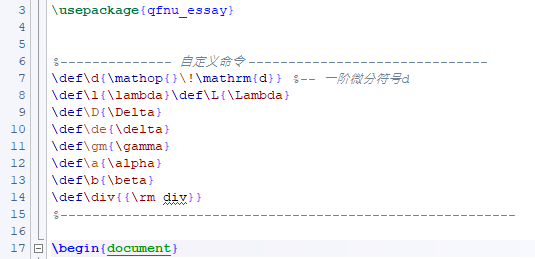
\includegraphics[width =4in]{Img/redefine.png}
\caption{自定义命令}   %--- 插图标题 ---
\label{pic: redefine} %--- 插图的引用标签---
\end{figure}
  \item 基本信息: 论文中英文标题, 专业中英文名称, 学号, 作者姓名, 指导教师姓名等.  见图\ref{pic: basic-info}.
\begin{figure}
\centering
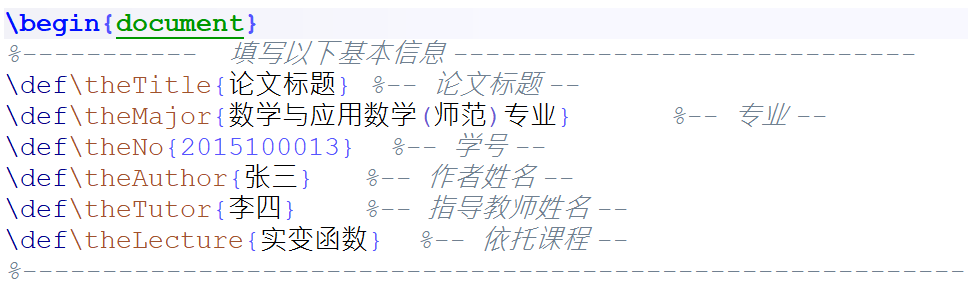
\includegraphics[width =4in]{Img/basic-info.png}
\caption{基本信息}   %--- 插图标题 ---
\label{pic: basic-info} %--- 插图的引用标签---
\end{figure}
  \item 中英文摘要和关键词.
  \item 正文内容.
  \item 参考文献. 列出的参考文献都要在正文中被引用, 否则不要出现.
\end{itemize}

 % 使用说明
\section{\LaTeX 示例}

读者应仔细查看这部分的tex源文件内容.

\subsection{定理环境}

下面是一个定义. 将对应的\LaTeX{}环境命令里的definition换成theorem, lemma, proposition, corollary,example, remark,就得到定理、引理、命题、推论、例、注等).
\begin{definition}[\cite{Liang-Xu-Auto18}]\label{Def: positive def matrix}
%------\begin{definition}[引用的定义所在的参考文献的标签] \label{给这个定义设置一个标签}
%----- 标签lable里的Def: positive def matrix是作者自己加上去的,为了方便交叉引用,加的标签最好有一定的意义,容易记忆
$n$阶实对称矩阵$A$为正定的,如果它所对应的二次型$X^T A X$是正定的,即对任意非零的$n$维列向量$X$, 有$X^T A X>0$.
\end{definition}



根据定义\ref{Def: positive def matrix} (注意这里的交叉引用方法), 我们有......

下面是性质,还包含一个列表的使用例子,注意列表编号的格式。
\begin{property}\label{Property: positive matrix}
如果$A$和$B$都是正定矩阵, 则有:
\begin{itemize}
  \item[(1)]$A+B$是正定矩阵;
  \item[(ii)]$kA$$(k>0)$是正定矩阵;
  \item[(bla)]blablabla;
  \item[1.]
  \item[i.]
  \item[A.]
\end{itemize}
\end{property}

以下是一个引理。
\begin{lemma}
设$E:\Bbb{R}^+ \to \Bbb{R}^+$ ($\Bbb{R}^+=[0,+\infty)$)是一个单调递减的函数且存在常数$T>0$,使得
$$\int_t^{\infty} E(s) \d s \leq TE(t),\quad \forall t\in \Bbb{R}^+,$$
则
$$E(t)\leq E(0) e^{1- \frac{t}{T}},\quad \forall t\geq T. $$
\end{lemma}

下面是一个定理及证明, 注意不等式(\ref{ineq-1})的交叉引用方法.
\begin{theorem}
设$E$是定义在$[0,\infty)$上的非负递减函数. 如果
\begin{equation}\label{ineq-1}  %----- 标签lable里的ineq-1是作者自己加上去的,为了方便交叉引用,加的标签最好有一定的意义,容易记忆
\int_S^{\infty} E(t) \d t \leq CE(S),\quad \forall S\geq S_0,
\end{equation}
其中$S_0$, $C$为固定常数, 则
$$E(t)\leq E(0)e^{1-\frac{t}{S_0+C}},\quad \forall t\geq 0.$$
\end{theorem}

\begin{proof}
若$0\leq S\leq S_0$, 由(\ref{ineq-1})式可知
\begin{eqnarray*}
  \int_S^{\infty} E(t)\d t &=& \int_S^{S_0} E(t)\d t +\int_{S_0}^{\infty} E(t)\d t\\
  &\leq &(S_0-S) E(S)+CE(S_0)\\
 &= &S_0 E(S) +CE(S)
\end{eqnarray*}
因此, 对$\forall S\geq 0$, 有
$$\int_S^{\infty} E(t) \d t \leq  (S_0+C)E(S).$$
由引理3得
$$E(t)\leq E(0)e^{1-\frac{t}{S_0+C}},\quad \forall t\geq 0.$$
\end{proof}
\begin{remark}
这里是一个注。
\end{remark}

\begin{theorem}[局部存在性与唯一性, \cite{Liang-Xu-Auto18}]  \label{Thm: local existence}
 假设\textbf{条件} 成立, 则存在依赖于初始二次能量~$\mathscr{E}(0)$ 的~$T>0$ 使得问题在时间区间~$(-\infty, T]$ 上有弱解. 另外, 我们有下面的能量恒等式成立:
\begin{eqnarray}
&&\mathscr{E}+\int_0^t\int_\Omega |u_t|^{m+1} \d x\d \tau-\frac12 \int_0^t\int_0^{-\infty}|\nabla w(\tau,s)|_2^2 \mu'(s)\d s\d \tau\nonumber\\
&&=\mathscr{E}(0)+\int_0^t\int_\Omega |u|^{p-1}uu_t\d x\d\tau,\label{4 quadratic energy identity}
\end{eqnarray}
\end{theorem}


下面是一个例.
\begin{example}
  这是一个例子.
\end{example}


\subsection{数学公式、符号的例子}

行列式的例子
\begin{equation*}
  |\lambda E- A|=
  \begin{vmatrix}
   \lambda-a_{11} & -a_{12} & -a_{13}&\cdots &-a_{1n} \\
    -a_{21} & \lambda-a_{22} & -a_{23} &\cdots & -a_{2n}\\
    \vdots & \vdots & \vdots&\ddots&\vdots \\
    -a_{n1} & -a_{n2} & -a_{n3} &\cdots& \lambda -a_{nn}
 \end{vmatrix}.
\end{equation*}

矩阵的例子
\begin{equation*}
A=(a_{ij})_{n\times n} =
\begin{pmatrix}
  a_{11} & a_{12} & a_{13} & \cdots & a_{1n}\\
  a_{21} & a_{22} & a_{23} &\cdots & a_{2n}\\
 \vdots & \vdots & \vdots & \ddots& \vdots\\
 a_{n1} & a_{n2} & a_{n3} &\cdots & a_{nn}
\end{pmatrix}.
\end{equation*}

方程组的例子
\begin{equation*}
\left\{   %------ 定界符是大括号{。 \left\{   与后面的\right. 对应
    \begin{aligned}
      &u_{tt}-\Delta u+|u_t|^{m-1}u_t=|u|^{p-1}u,\quad (x,t)\in \Bbb{R}^n\times (0,\infty),\\
      &u(0,x)=u_0(x),\quad u_t(x,0)=u_1(x),
      \end{aligned}
\right.
\end{equation*}

\begin{equation*}
\left\{
   \begin{array}{rl} %---- 分为两列,第一列右对齐(r=right),第二列左对齐(l=left)
      -x & \text{if } x < 0,\\
       0 & \text{if } x = 0,\\
       x & \text{if } x > 0.
\end{array}
\right.
\end{equation*}


长公式
\begin{eqnarray*}
J(\psi_t(v);t)&=&\frac{p-2}{2p}(|\nabla \psi_t(v)|_2^2+b|\psi_t(v)|_2^2)+\frac1p I(\psi_t(v);t) \\
                &=&\frac{p-2}{2p}s^2(v;t)\|v\|^2 \\
                &=&\frac{p-2}{2p}(k(t))^{-\frac{2}{p-2}}\|v\|^{\frac{2p}{p-2}}.
\end{eqnarray*}
\begin{eqnarray*}
  &       &\frac{\gamma_a^p\left(2\rho(0)\right)^{1-\frac{p}{2}}}{\left(p-2\right)k(T_3)}\leq T^* \\
  &\leq & T_3:= \frac{8(p-1)(a\l_1+1)\rho(0)}{(p-2)^2[(p-2)(b+\l_1)\rho(0)-p(a\l_1+1)J(u_0;0)]};
  \end{eqnarray*}


 一个具有斜线表头的表格
 \begin{center}
\begin{tabular}{|c|c|c|} %------ 三列的列表,每列都居中对齐
  \hline
  % after \\: \hline or \cline{col1-col2} \cline{col3-col4} ...
  \diagbox{$X$}{$Y$} & $a$ & $b$ \\
  \hline
    $c$ & 1   &0 \\
   \hline
  $d$ & 0 &1 \\
  \hline
\end{tabular}
 \end{center}





三线表
\begin{table}[htbp]
\centering
 \caption{理论计算得到的PZT运动一个周期内干涉条纹数}
 \label{tab:theory}
 \begin{tabular}{ccc}
  \toprule
  图2.12、 2.13 & 振动幅度$(p-p)$ $(\mu m)$ & 理论计算的条纹数 \\
  \midrule
 (a) & 0.7$\mu m$ & 2.2 \\
 (b) & 1.3$\mu m$ & 4.1 \\
 (c) & 2$\mu m$ & 6.3 \\
  \bottomrule
 \end{tabular}
\end{table}

 % latex示例
\section*{\heiti\xiaosihao 致谢}
\phantomsection\addcontentsline{toc}{section}{致谢}

本文的写作过程中,得到了李四老师的悉心指导与修改, 在此表示感谢.

%参考文献
\references{
  \bibitem{jiang-06}  %jiang-06是自己为本条参考文献添加的标签
  姜国. 正定矩阵的判定及性质[J]. 湖北师范学院学报(自然科学版), 2006(01): 97-100.

  \bibitem{LiLiqun-17}
  李立群. 正定矩阵及其应用[J]. 山东农业工程学院学报, 2017, 34(07): 28-30.

  \bibitem{Liang-Xu-Auto18}
  Xiao Liang, JuanJuan Xu. Control for networked control systems with remote and local controllers over unreliable communication channel[J]. Automatica, 2018, 98(2018): 86-94.
} % 致谢/参考文献
